\begin{center}
\og \textit{La Croix : chemin de notre salut} \fg
\end{center}

La passion du Christ est très dramatique. Elle dépasse l’entendement humain. C’est une histoire où se rencontrent la bassesse de l’homme et la grandeur de Dieu. En écoutant cette passion, on ressent un sentiment d’indignation devant l’odieux procès qui conduit à la condamnation d’un innocent. Mais en même temps, on découvre par ailleurs le profond respect et l’immense gratitude envers le Fils de Dieu qui nous a aimé jusqu’au bout, au prix de sa vie.
La croix du Christ, signe d’amour et signe de notre salut. Elle reste pour chacun de nous un mystère.

En ce Vendredi Saint, nous nous réunissons pour méditer sur la Passion-Mort et Résurrection du Christ. Sa vie terrestre n’a pas été longue mais elle a été parfaitement réussie parce qu’elle était centrée sur l’Amour. Elle n’a trouvé sa plénitude qu’au-delà de la mort, dans la résurrection et la communion définitive avec le Père. C’est bien là, le symbole de notre propre aventure personnelle. Et pourtant… nous oublions trop souvent que, sur cette terre, nous ne sommes que des pèlerins. Nous avons trop tendance à nous installer. Nous savons que la Vie Éternelle commence sur terre, mais nous oublions que son terme se situe dans la rencontre définitive de Dieu.
Pour progresser dans l’intelligence du mystère de la croix, il ne suffit pas d’acclamer la croix ou de la vénérer. Ce n’est pas non plus de discuter à perte de vue sur ce mystère. Le plus important c’est de prendre modèle sur le Christ : Il n’a pas attendu le Calvaire pour donner sa vie. Il l’a fait jour après jour au hasard des rencontres, chaque fois qu’il s’est mis au service des petits, des malades et des pauvres.
Beaucoup ont compris que la meilleure manière de porter sa croix c’est de porter celle des autres,
\begin{wrapfigure}{l}{0.1\textwidth}
\vspace{-0.5cm}
\centering
	%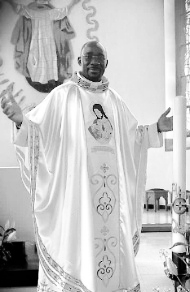
\includegraphics[width=0.1\textwidth]{standing_daniel.png}
	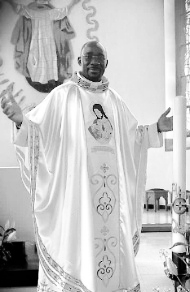
\includegraphics[scale=1.2]{standing_daniel.png}
\end{wrapfigure}
c’est de faire renaître et aider à renaître à l’espérance tous ceux qui sont méprisés, asservis, malades, découragés. C’est ainsi que nous sommes appelés à célébrer la croix du Christ.

En ce Vendredi Saint, les uns pour les autres,
nous prierons
l’Esprit Saint pour qu’il ouvre chacun de nos cœurs à l’intelligence de plus en plus grande de ce mystère d’amour qu’est le mystère de la Croix. Et c’est alors seulement que nous pourrons chanter en toute vérité : \og Victoire ! Tu règneras. Ô croix, tu nous sauveras \fg.



\begin{flushright}
Bonne montée vers Pâques !\\
\textit{Père  Daniel  ETTÉ}
\end{flushright}
